% ==============================================================================
% Chapter 3: Stakeholders, Requirements (FR/NFR) & Operational Use Cases
% ==============================================================================
\chapter{אפיון דרישות המערכת, בעלי עניין ותרחישי ייחוס מבצעיים}
\label{ch:requirements}

\section{מיפוי בעלי העניין ומערכת האיזונים המוסדית}
מערכת לאומית לניטור מידע ציבורי אינה פועלת בחלל ריק; הצלחתה תלויה בהפרדת תפקידים חדה בין הגורם המתפעל הטכנולוגי, הרשות המפקחת על טוהר הבחירות, הערכאה המשפטית המוסמכת, כלי התקשורת והציבור הרחב. טבלה~\ref{tab:stakeholders} מפרטת את ששת בעלי העניין המרכזיים של \en{CivicShield AI}, סמכויותיהם, הדרישות שהם מציבים בפני המערכת, והבלמים המונעים ניגוד עניינים ביניהם.

{\renewcommand{\arraystretch}{1.35}
\begin{table}[htbp]
\centering
\caption{מטריצת בעלי העניין, סמכויות ואיזונים מוסדיים}
\label{tab:stakeholders}
\begin{tabularx}{\textwidth}{|p{2.9cm}|p{3.0cm}|X|p{3.1cm}|}
\hline
\textbf{\textcolor{CivicNavy}{בעל עניין}} & \textbf{\textcolor{CivicNavy}{תפקיד מוסדי}} & \textbf{\textcolor{CivicNavy}{דרישה מרכזית מהמערכת}} & \textbf{\textcolor{CivicNavy}{מנגנון ריסון ובקרה}} \\ \hline
ועדת הבחירות המרכזית (\en{CEC}) & הגוף הסטטוטורי לטוהר ההליך & קבלת התראות \en{FIMI} מוקדמות והמלצות לחיסון תודעתי בלתי מפלגתי. & החלטות אכיפה טעונות אישור יו"ר הוועדה (שופט עליון). \\ \hline
מערך הסייבר הלאומי (\en{INCD}) & הגנת תשתיות וניטור תקיפה & זיהוי קמפייני בוטים, תשתית שרתים עוינת וחסימת דומיינים מתחזים. & איסור איסוף תוכן אישי של אזרחים; מיקוד בתשתיות \en{FIMI}. \\ \hline
משרד המשפטים והייעוץ המשפטי & הגנת זכויות יסוד וחוקתיות & אימות שקיפות, שיוויון פוליטי ותאימות להלכת דמוקרטיה מתגוננת. & זכות וטו קשיחה על פתיחת תיקים וחתימה משולשת מחייבת. \\ \hline
מערכות תקשורת ועיתונות & מתווך מקצועי לציבור & קבלת התראות אימות פורנזי על \en{Deepfake} וחטיפת סדר יום בזמן אמת. & הנגשת ראיות פתוחות ללא תכתיב עריכתי ממשלתי. \\ \hline
האקדמיה והחברה האזרחית & ביקורת חיצונית עצמאית & גישה למדדי מאקרו אנונימיים (\en{$\epsilon$-DP}) לצורך פיקוח מחקרי. & קוד פתוח חלקי לביקורת דחיית הטיות (\en{Fairness Audit}). \\ \hline
האזרח והבוחר הישראלי & הריבון הדמוקרטי & הגנה מפני הונאה מבלי להישלט או להיות מצונזר בשיח הלגיטימי. & חסימת מעקב פרטי; שקיפות מלאה על הודעות חיסון. \\ \hline
\end{tabularx}
\end{table}}

\section{מפרט דרישות פונקציונליות (\en{FR-01} עד \en{FR-15})}
הדרישות הפונקציונליות של \en{CivicShield AI} חולקו לשלוש קבוצות תפעוליות המשתלבות באופן ישיר עם ועדת סוכני ה-\en{AI} (פרק~\ref{ch:architecture}) ועם המודלים המתמטיים (פרק~\ref{ch:math}).

\subsection{קבוצה א': קליטה, ניטור וזיהוי פורנזי (\en{FR-01} עד \en{FR-05})}
קבוצה זו אחראית על צינור האיסוף הגלוי (\en{Public OSINT Streaming}) והסקת תכונות ברמת פוסט, חשבון ומדיה:

{\renewcommand{\arraystretch}{1.35}
\begin{table}[htbp]
\centering
\caption{דרישות פונקציונליות — ניטור, קליטה וזיהוי פורנזי (FR-01 עד FR-05)}
\label{tab:fr_group_a}
\begin{tabularx}{\textwidth}{|p{1.8cm}|p{3.4cm}|X|p{2.0cm}|}
\hline
\textbf{\textcolor{CivicNavy}{מזהה}} & \textbf{\textcolor{CivicNavy}{שם הדרישה}} & \textbf{\textcolor{CivicNavy}{פירוט תפעולי מחייב}} & \textbf{\textcolor{CivicNavy}{עדיפות}} \\ \hline
\en{FR-01} & קליטת זרמי \en{OSINT} פומביים & התחברות בזמן אמת ל-\en{APIs} פומביים של רשתות חברתיות, ערוצי טלגרם פתוחים ופורטלי חדשות, ללא גישה למסרים פרטיים. & חובה (\en{P0}) \\ \hline
\en{FR-02} & סינון ומיסוך פרטיות בכניסה & הפעלת מסנן מיסוך מזהים (\en{PII Redaction}) והזרקת רעש \en{$\epsilon$-DP} מיד בעת האינדוקס לזיכרון המערכת. & חובה (\en{P0}) \\ \hline
\en{FR-03} & גילוי התנהגות מתואמת (\en{CIB}) & אשכול של חשבונות לפי חתימת זמן פרסום (\en{$\Delta t < 2s$}), מבנה גרף שיתוף זהה (\en{Co-Sharing}) ומוטיבים חוזרים \cite{pacheco2021}. & חובה (\en{P0}) \\ \hline
\en{FR-04} & סיווג מסגור אנטמן אוטומטי & ניתוח טקסטואלי בעברית ובערבית של ארבע פונקציות המסגור: הגדרת בעיה, אשם, שיפוט מוסרי ופתרון \cite{entman1993}. & גבוהה (\en{P1}) \\ \hline
\en{FR-05} & גלאי \en{Deepfake} מולטי-מודאלי & ניתוח מקבילי של ספקטרוגרמת קול, עקביות אופטית של שפתיים ועיניים, ומטא-דאטה קריפטוגרפי (\en{C2PA}). & חובה (\en{P0}) \\ \hline
\end{tabularx}
\end{table}}

\subsection{קבוצה ב': מידול תודעתי, קיטוב וחיזוי (\en{FR-06} עד \en{FR-10})}
קבוצה זו מחברת את הסוכנים האבחנתיים למנוע הסימולציות הכמותיות, המאפשר מעבר מתצפית סטטית לתחזית דינמית:

{\renewcommand{\arraystretch}{1.35}
\begin{table}[htbp]
\centering
\caption{דרישות פונקציונליות — מידול אפידמיולוגי וחיזוי קיטוב (FR-06 עד FR-10)}
\label{tab:fr_group_b}
\begin{tabularx}{\textwidth}{|p{1.8cm}|p{3.4cm}|X|p{2.0cm}|}
\hline
\textbf{\textcolor{CivicNavy}{מזהה}} & \textbf{\textcolor{CivicNavy}{שם הדרישה}} & \textbf{\textcolor{CivicNavy}{פירוט תפעולי מחייב}} & \textbf{\textcolor{CivicNavy}{עדיפות}} \\ \hline
\en{FR-06} & מנוע הדבקה תודעתית (\en{SIRI}) & שיערוך מקוון של קצב ההדבקה \en{$\beta(t)$}, מקדם ההתרבות \en{$R_0$} ושיעור החשיפה הצפוי ב-24 השעות הקרובות. & חובה (\en{P0}) \\ \hline
\en{FR-07} & מדידת זליגה בין-ערוצית & מעקב אחר מעבר נרטיבים מערוצי קצה בטלגרם אל כלי תקשורת המוניים וחישוב זמן השיהוי (\en{Spillover Lead Time}). & גבוהה (\en{P1}) \\ \hline
\en{FR-08} & מדד קיטוב ותיבות תהודה & הרצת מודל \en{Hegselmann-Krause} רציף להפקת אינדקס דו-קוטביות (\en{Bimodality}) וזיהוי תופעות ספירלת השתיקה. & גבוהה (\en{P1}) \\ \hline
\en{FR-09} & דירוג סמכותיות אפיסטמית & אימות צולב בין טענות הנוגעות לנהלי הצבעה לבין מאגר החוקים והדיווחים המאומת של ועדת הבחירות המרכזית. & חובה (\en{P0}) \\ \hline
\en{FR-10} & שיוך מבצע השפעה (\en{FIMI Attribution}) & שילוב אותות רשתיים, תבניות תרגום מכונה מובהקות ולוחות זמנים גאוגרפיים להערכת סבירות למעורבות שחקן זר. & בינונית (\en{P2}) \\ \hline
\end{tabularx}
\end{table}}

\subsection{קבוצה ג': חוקתיות, חיסון תודעתי והנגשה (\en{FR-11} עד \en{FR-15})}
קבוצה זו מגדירה את ממשקי ההתערבות המותרים בלבד, תוך איטום קשיח בפני פעולה אוטומטית פולשנית:

{\renewcommand{\arraystretch}{1.35}
\begin{table}[htbp]
\centering
\caption{דרישות פונקציונליות — הגנה חוקתית, חיסון תודעתי ושקיפות (FR-11 עד FR-15)}
\label{tab:fr_group_c}
\begin{tabularx}{\textwidth}{|p{1.8cm}|p{3.4cm}|X|p{2.0cm}|}
\hline
\textbf{\textcolor{CivicNavy}{מזהה}} & \textbf{\textcolor{CivicNavy}{שם הדרישה}} & \textbf{\textcolor{CivicNavy}{פירוט תפעולי מחייב}} & \textbf{\textcolor{CivicNavy}{עדיפות}} \\ \hline
\en{FR-11} & מחסום מניעת צנזורה אוטומטית & חסימה מוחלטת ברמת התוכנה והחומרה של כל קריאת \en{API} להסרת תוכן ללא מנגנון חתימה אנושי משולש. & חובה (\en{P0}) \\ \hline
\en{FR-12} & מחולל חיסון תודעתי (\en{Prebunking}) & הצעת 3 חלופות של הודעות אזהרה קוגניטיביות ניטרליות החושפות טכניקת מניפולציה ללא נקיטת עמדה מפלגתית. & חובה (\en{P0}) \\ \hline
\en{FR-13} & חתימה משולשת (\en{Triple-Key Quorum}) & תהליך אישור מבוזר הדורש חתימות \en{Ed25519} של נציג שופט, מערך הסייבר ומפקח ציבורי לפני כל פעולה פורמלית. & חובה (\en{P0}) \\ \hline
\en{FR-14} & יומן ביקורת בלתי ניתן לשינוי & תיעוד שרשרת הנימוקים (\en{ReAct Trace}) של כל סוכן לתוך יומן \en{Append-Only Merkle Log} לביקורת שיפוטית. & חובה (\en{P0}) \\ \hline
\en{FR-15} & דשבורד שקיפות פתוח לציבור & הצגת תרשימי מגמת בוטים אנונימיים ותמרורי חיסון מאושרים באתר ציבורי גלוי בזמן אמת. & גבוהה (\en{P1}) \\ \hline
\end{tabularx}
\end{table}}

\section{דרישות לא-פונקציונליות (NFRs) ומדדי סף הנדסיים}
מעבר ליכולת האנליטית, יום בחירות מייצר עומס תנועה בלתי סדיר וקיצוני של תגובות רשת, סרטוני וידאו ותעבורת חדשות. לפיכך, המפרט הלא-פונקציונלי של \en{CivicShield AI} (טבלה~\ref{tab:nfrs}) מציב תקני שרידות, אבטחה וזמני תגובה המחייבים תכנון הנדסי מבוסס ענן היברידי ומאיצי \en{GPU}.

{\renewcommand{\arraystretch}{1.35}
\begin{table}[htbp]
\centering
\caption{מפרט דרישות לא-פונקציונליות (NFR-01 עד NFR-08)}
\label{tab:nfrs}
\begin{tabularx}{\textwidth}{|p{1.9cm}|p{3.0cm}|p{3.1cm}|X|}
\hline
\textbf{\textcolor{CivicNavy}{מזהה}} & \textbf{\textcolor{CivicNavy}{קטגוריה}} & \textbf{\textcolor{CivicNavy}{יעד מדיד (\en{SLA})}} & \textbf{\textcolor{CivicNavy}{שיטת אימות ובקרה}} \\ \hline
\en{NFR-01} & השהיית עיבוד (\en{Latency}) & ממוצע \en{$< 250\,\text{ms}$} ב-\en{12k EPS} & מודל תורים \en{M/M/c} עם \en{34} קבוצות שרתים (פרק~\ref{ch:math}). \\ \hline
\en{NFR-02} & זמינות יום הבחירות & זמינות \en{99.99\%} (\en{Active-Active}) & שרידות מרובת-אזורים (\en{Multi-AZ}) ו-\en{Failover} תחת 15 שניות. \\ \hline
\en{NFR-03} & דיוק זיהוי \en{Deepfake} & \en{$\text{AUC} > 0.96$}, \en{$\text{Precision} \ge 0.90$} & מניעת התראות שווא המפעילות את השער החוקתי שלא לצורך. \\ \hline
\en{NFR-04} & הגנת פרטיות & תקציב פרטיות \en{$\epsilon \le 1.2$} & הוכחה מתמטית להיעדר זיהוי חוזר (\en{Re-identification}) בדשבורדים. \\ \hline
\en{NFR-05} & איזון פוליטי והטיה & פער דיוק בין גושים \en{$< 1.5\%$} & מבחני כיול דו-שבועיים על קורפוס מבוקר מכלל הקשת הפוליטית. \\ \hline
\en{NFR-06} & שפה ומולטי-לינגואליות & עברית, ערבית, רוסית, אמהרית & תמיכה מלאה בסלנג פוליטי, דיאלקטים וזיהוי תעתיקים מקודדים. \\ \hline
\en{NFR-07} & שקיפות והסברתיות & \en{100\%} נימוק ראיות (\en{XAI}) & כל התראה כוללת מקורות גולמיים, ציון ביטחון ומפת פונקציות אנטמן. \\ \hline
\en{NFR-08} & עמידות בהתקפת נגד & סיכול \en{Prompt Injection} & שכבת אימות תחבירית וארגז חול מבודד לסוכנים המנתחים טקסט זר. \\ \hline
\end{tabularx}
\end{table}}

\section{תרחישי ייחוס מבצעיים (Operational Use Cases)}
להמחשת האינטראקציה המבצעית בין הדרישות, נבחן ארבעה תרחישי קיצון של שבוע הבחירות, הממחישים כיצד פועלת ועדת הסוכנים מול איומי תודעה ריאליים.

\begin{archbox}[תרחיש ייחוס UC-01: נחיל בוטים מתואם בטלגרם להרתעת מצביעים (72 שעות לפני הקלפי)]
\textbf{תיאור האיום:} 480 ערוצים וקבוצות פתוחות מפיצים תוך 9 דקות שמועה זהה עם פוסטרים גרפיים הטוענים כי "מערך המחשוב של הקלפיות בדרום נפרץ ועשרות אלפי קולות ייגרעו".\\
\textbf{תגובת המערכת:} רכיב \en{FR-03} מאתר מתאם פרסום של מתחת ל-1.8 שניות ומזהה טביעת לשון תרגומית זהה. תוצר הסימולטור (\en{FR-06}) קובע מקדם הדבקה מוקדם \en{$R_0 = 4.2$}. סוכן הבקרה החוקתי מוודא כי לא מדובר בביטוי לגיטימי של מפלגה מוכרת אלא בפרופיל \en{FIMI} מובהק. תוך 22 דקות מנפיקה ועדת הבחירות קמפיין \en{Prebunking} ממוקד (\en{FR-12}) המסביר כיצד זייפנים מנצלים גרפיקות פחד ללא מקור משפטי, ותוקע טריז לפני חדירת הנרטיב למהדורות החדשות.
\end{archbox}

\begin{archbox}[תרחיש ייחוס UC-02: הפצת Deepfake קולי של מועמד מוביל בבוקר הבחירות]
\textbf{תיאור האיום:} בשעה 08:15 בבוקר הבחירות עולה קובץ אודיו ב-\en{WhatsApp Public Channels} וב-\en{X}, שבו נשמע כביכול יו"ר רשימה מובילה מורה לפעיליו לשבש הצבעה באזורי מיעוטים.\\
\textbf{תגובת המערכת:} סוכן הפורנזיקה (\en{FR-05}) מזהה חוסר רציפות ספקטרלית בתדרי \en{4--8 kHz} האופיינית לסינתזה עצבית והיעדר נשימות טבעיות, תוך סריקה צולבת המגלה היעדר חתימת שידור \en{C2PA} ותאום העלאה של 1,200 בוטים בדקה הראשונה. שילוב הראיות הבייסיאני מניב הסתברות זיוף של \en{97.4\%}. ההתראה מועברת בשידור חי לתאי העיתונאים המרכזיים (\en{NFR-07}) ומונעת שידור מוטעה במהדורות הצהריים, לצד פתיחת בקשת הסרה בחתימה משולשת (\en{FR-13}) לרשתות החברתיות.
\end{archbox}

\section{ניתוח כמותי: בלימת זליגת סדר היום והסטת המסגור (תוצאות סימולציה)}
אחת ההבטחות האקדמיות המרכזיות של \en{CivicShield AI} היא בלימת \textbf{קביעת סדר היום הבין-תקשורתית ההפוכה} (פרק~\ref{ch:theory}). איור~\ref{fig:agenda_framing_shift} מציג את ממצאי ההרצה הסימולטיבית לאורך חלון של 72 שעות מהזרקת זרע המניפולציה הראשוני.

בגרף השמאלי (פאנל \en{A}) מודגמת השתלשלות הנרטיב ללא הגנה מול פעולת המגן: הזרם השולי בטלגרם (\en{Fringe Channels}) מגיע לשיא מוקדם סביב השעה ה-10 (\en{t=10h}), ואחריו מגיעה התפרצות משנית של הגברת בוטים סביב השעה ה-22 (\en{t=22h}), הגוררת חדירה מסיבית לתקשורת המרכזית עד סביב השעה ה-28–38. לעומת זאת, כאשר \en{CivicShield AI} מזהה את האנומליה כבר ב-\en{t=8h} ומזניקה התערבות \en{Prebunking} ממוקדת, שיא החדירה לתקשורת המרכזית נבלם בעקומת סף שטוחה ברמה של כ-13 נקודות בולטות בלבד — הפחתה דרמטית של ההד המערכתי.

בגרף הימני (פאנל \en{B}) נמדדת הצלחת הבלימה על פי ארבע פונקציות המסגור של אנטמן \cite{entman1993}: ללא הגנה, אימוץ מסגרת "הבעיה" מגיע ל-\en{78\%}, האשמה סיבתית ל-\en{82\%}, פאניקה מוסרית ל-\en{88\%} ואי-אמון מוסדי ל-\en{74\%}; הפעלת החיסון המוקדם של המערכת מצניחה שיעורים אלה ל-\en{24\%}, \en{19\%}, \en{27\%} ו-\en{16\%} בהתאמה — פגיעה ישירה ביעילות התודעתית של התוקף מבלי למחוק שיח לגיטימי.

\begin{figure}[htbp]
\centering
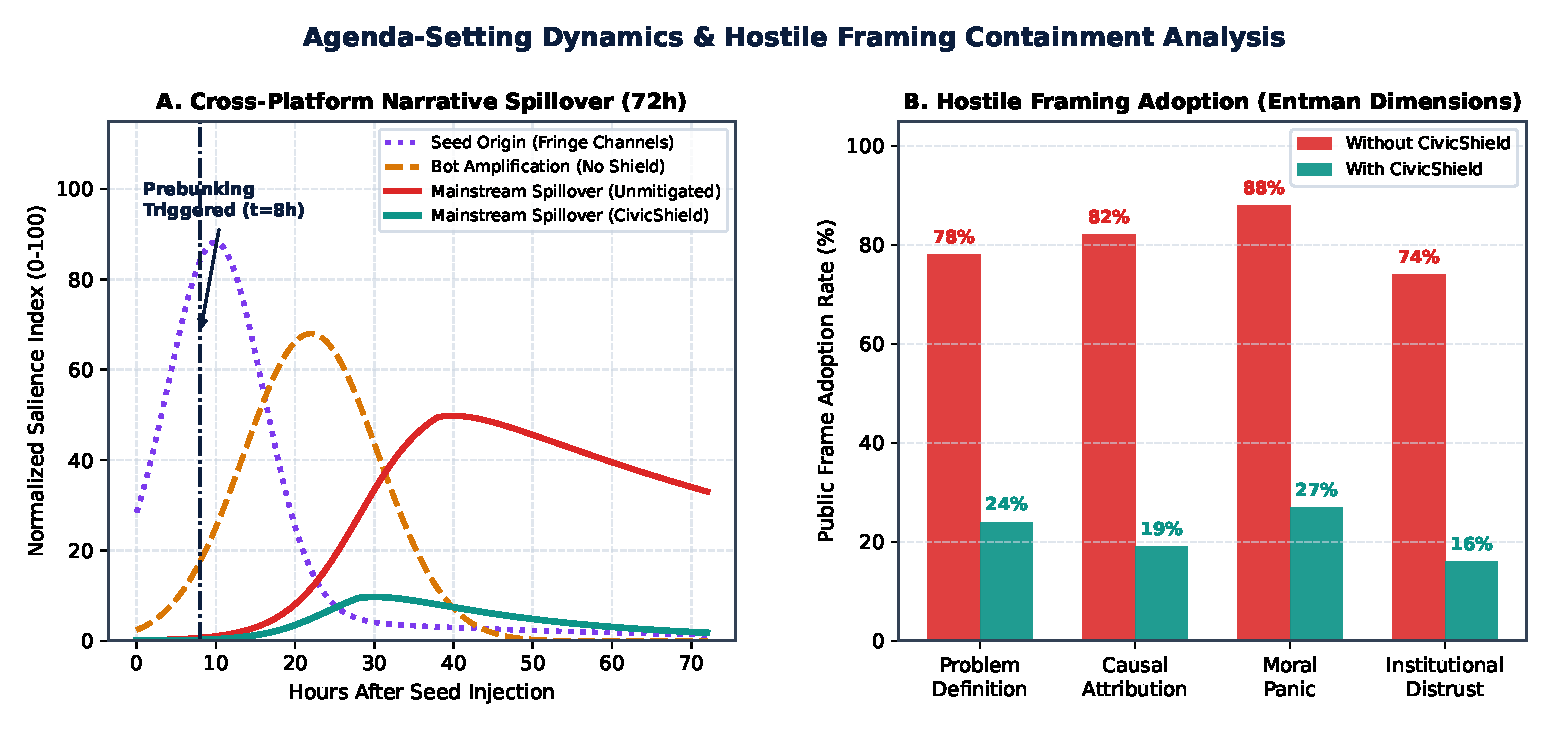
\includegraphics[width=0.95\textwidth]{figures/fig4_agenda_framing_shift.pdf}
\caption{דינמיקת זליגת סדר יום בין פלטפורמות ובלימת אימוץ מסגרות עוינות לפי מימדי אנטמן}
\label{fig:agenda_framing_shift}
\end{figure}

בהמשך לכך, תרחישי הייחוס \en{UC-03} (זיהוי חטיפת סדר יום בתוך תקופת השתיקה של 48 שעות טרם הבחירות) ו-\en{UC-04} (פריסת מסר חיסון ניטרלי מתוקף מדעית לכלל מפלגות הקואליציה והאופוזיציה במידה שווה) משלימים את המעטפת המבצעית של \en{CivicShield AI}: המערכת משמשת רדאר ציבורי א-פוליטי שאינו מתערב בהתמודדות הדמוקרטית עצמה, אלא שומר על תקינות כללי המשחק ועל אמינות המרחב האפיסטמי שבו מוכרעת התחרות.
